\chapter{Research}

The outline of this research report is as follows: First the problem domain is explained, which entails a description of the domain and an analysis. Based on the analysis, a research question was formulated that embodies the main objectives, followed by a list of project requirements. After that follows a technical analysis that facilitates the requirements. Finally the project's implementation methodology is illustrated.

Secondly the project's requirements are listed, together with some background information about how they came to be. The final part of this research report provides us with the optimal solution for our problem.


\section{Problem Domain} % (fold)
\label{sec:problem_domain}

% section problem_domain (end)

Within the following section the problem domain will be described and analyzed in terms of what the problem domain is exactly, who the identified stakeholders are and what the scope and objectives should be. A summary of conducted interviews is given at the end of this section.

\subsection{Domain Description} % (fold)
\label{sub:problem_description}

The goal of this project is the creation and implementation of a prototype for a `Virtual Assistant' application, which helps students and researchers write a report, thesis or dissertation. The initial idea entailed that the Virtual Assistant should provide its users with the ability to choose a layout template, allow for scheduling and feedback, and give suggestions or tips about how to write a report, thesis or dissertation. This project should be created in the form of either native desktop software, a web application, or a mobile application. The final prototype would eventually be released as open source software.

\subsection{Domain analysis} % (fold)

One of the key aspects that need to be well-researched for this project is the domain analysis. The domain analysis illustrates all the different types of roles involved with the problem domain (i.e. the stakeholders), and what their interests are. First all the stakeholders involved with the domain are listed, after which the definition of the scope is given. To end the domain analysis, a summary of conducted interviews with people that embody relevant roles is given.

\subsubsection{Stakeholders} % (fold)

Below the different stakeholders are identified, which roles they can take, and what their main interests are within our problem domain.

\paragraph{Client: TU Delft Library} The TU Delft Library is the entity that requested this project, and is therefor the client. They expect a prototype of a product that meets their requirements.

\paragraph{Users: Students and Researchers} The use of this product is aimed at students, and researchers, which makes them a subset of our users. They want a product that is easy to use and helps them with writing a report/thesis/dissertation.

\paragraph{Users: Reviewers} The use of this product is also aimed at reviewers who, together with the students and researchers, complete the set of users. They also want a product that is easy to use and facilitates them in reviewing a report/thesis/dissertation.

\paragraph{Contributors: Open Source Developers} Our client requested that our final prototype version be released as an open source project. This means that at some point in the future other developers are going to improve upon our prototype. With this in mind, some design ideals and constraints need to be introduced that will make it easier for them to add code in the future.

\subsubsection{Scope \& Objectives}

The scope of the domain is set for the use-case of students who are writing a Bachelor project final report. One obvious reason for this scope is that this project is also a Bachelor final project, which will also include the process of writing a final report. This means that we, as the developers, will have affinity with the scope, which should imply an advantage within the design. Another reason is that there are plainly too many different cases and subjects within the problem domain to serve all of them accordingly within the given deadlines.
The main objective is the creation of an on-line environment that acts as a support for students who are writing a report/thesis/dissertation. It should provide the students with suggestions, tips, sources and other relevant information. It should also provide a platform where there is an interaction between students and their peers or superiors (in this case a teacher, coach or supervisor), and where they can exchange feedback with each other.

\subsubsection{Interview result analysis} % (fold)

The most challenging part in this project is understanding how the application can provide suggestions, tips, sources and other relevant tools and information to the students. In order to get a more detailed comprehension of this part within the problem domain, a couple of interviews with stakeholders were conducted. The purpose of these interviews was to gain a better understanding of tools and information that users wish to have at hand. The interviews were conducted from three stakeholders; a student who is writing an article, a reviewer which reviews an article and someone who is an expert in providing information on writing a scientific articles. The summary of these interviews can be found in appendix \ref{interview}.

\section{Research Question}

The context of this project is to build an application that acts as a virtual assistant which can help Bachelor students write their article/report in a correct manner. In order to design a robust and reliable software application, a research question needs to be formulated in order to do the technical research and to come up with a feasible and optimal solution for developing a prototype application.\\\\

During the first meeting that involved both the client and coach, in which the latter has persuaded us to develop a web application. Throughout the rest of this research report, the assumption that a web application is most likely the best choice of platform is made, whereas the research itself is intended to find out whether this assumption is correct, and if so, why it would be an ideal choice. \\\\

The main research question is formulated as follows: `How do we build a reliable and robust web application prototype that is able to assist students in writing an article or report, and is also able to guide them in such a way that they are able to write an article or report in a correct and efficient manner within the time constraint that is given to them? '

\section{Project Requirements}
\label{req}

The project's requirements form up the backbone to a project. They are agreed upon in accordance with the client and coach. It is imperative that these requirements are met at the end of the implementation. In this section we first explain about how the requirements were reached, and then list the functional and technical and usability requirements of the project.

\subsection{Formulating the requirements} % (fold)
\label{sub:subsection_name}
The analysis of the requirement proved to be a very important step within the project, as it allowed for the creation of a concrete list of functional, technical and usability requirements for. In appendix \ref{mindmap}, a mind-map is illustrated showing a summary of all the tools and functionalities that were considered during the synthesis of the project's requirements.

% subsection subsection_name (end)

\subsubsection{Initial Meeting with the Client, Coach and the Developers} % (fold)
\label{sub:meeting_client_coach_developer_team_meeting_}

An introductory meeting was organized by us, which involved both the coach and the client. The main idea behind this meeting was to introduce all the members that were involved within the project and, as the initial idea of the Virtual Assistant still had some rough edges at this point, also discuss the features that should be implemented within the project. The coach could then immediately evaluate the feasibility of the project to be completed in 12 weeks.\\
The meeting allowed for a list of initial requirements to be made, which made the idea of the application prototype more concrete for everyone involved. As a final remark it was also stated by the client that the prototype had to have a feature that would allow for usage analytics and usage of information that would be provided by \url{tulib.tudelft.nl/}.\\ 

% subsection meeting_client_coach_developer_team_meeting_ (end)


\subsection{Functional Requirements} % (fold)
\label{sub:functional_requirement}

Below is a list of functional requirements that the application should meet:

\begin{enumerate}
	\item Multiple Users: Each project created by one user can be joined by multiple other users, where none or more joining participants can be attributed owner privilege. The creator of the project will receive owner privilege by default. The application should also facilitate reviews from supervisors or other members.
	\item Template: The application will provide several templates for the user, or allow the user to upload his or her own template.
	\item Schedule: There has to be a module in which the users can schedule their writing progress according to their chosen template.
	\item Propose Suggestions/Tips: The system should be able to suggest tips and information to the user on how to write specific sections.
	\item Send/Receive Feedback: The application should facilitate feedback on a report written by a student from a reviewer.
	
	\item Upload/Download Document: The application should allow for the ability to upload a document to the application or download a document from a project.
	\item Built-in Chat mechanism: It should be possible to display the feedback from a reviewer and create an environment to discuss about specific submission. 
	\item Versioning : Keep track of the versions of publications that a user has uploaded.
	\item Logging : Save the user's records in a separate log file for usage analytics.
\end{enumerate}

% subsection functional_requirement (end)
\subsection{Technical Requirements} % (fold)
\label{sub:technical_requirements}

Besides the functional requirements, which illustrate how the system should work in usage, there are also some technical requirements that illustrate how the system should be built. These technical requirements are listed below:

\begin{enumerate}
	\item Campus ID authentication: allow login with TUDelft netID
	\item Google sign up/in mechanism: allow login with a Google account
	\item Mendeley library sharing: allow users within a project to share their references/citations.
	\item Released as Open Source
 	\item System should be fully tested 
\end{enumerate}

% subsection technical_requirements (end)
\subsection{Usability Requirements} % (fold)

Finally there are also some usability requirements that should be met in order to guarantee a user-friendly application:

\label{sub:usability_requirements}
\begin{enumerate}
	\item The application must be fully functional on modern web browsers
	\item Efficient in use: System must facilitate efficiency of use for the user by providing usage information
	\item Intuitiveness: The User Interface must be intuitive and easy to use
\end{enumerate}
% subsection usability_requirements (end)
\newpage
\section{Technical Analysis} % (fold)

Now that the requirements are set, and the research question has been formulated, it is now possible to translate the features into a technical environment. In this section we illustrate our findings, and justify our choices in terms of tools, deployment, architecture design and system components.

\subsection{Why a web application?}
One of the main ideas that has been advised by our coach is the creation of a web application for the project. The justification for this is ease of usability and compatibility across several platforms. Web applications are also exempted from platform-specific updates, whereas now one single update on the web application immediately reaches all of our users at once. When a web application is used, users can access the exact same content from different computers or mobile devices.
\subsection{Objectives}
There are various frameworks available for the implementation of a web application. The choice of a specific framework usually depends on the context and objectives of the project itself. This project entails the development of a prototype within a time constraint of 11 to 12 weeks, which persuaded us to use a full stack framework. A full stack framework should allow us to focus primarily on techniques that allow for to perform rapid prototyping, generate quality code and provide good documentation all of which meet the clients requirements. The following features should facilitate reaching the stated objectives during the development phase.

\begin{enumerate}
	\item \textbf{a Full-Stack framework}: A framework that already contains all the basic utilities to create and run an application, with the option to connect or import external entities.
	\item \textbf{Rapid Prototyping}: Convert the client's requirements into a prototype in a fast way so it can be immediately reviewed and refined for the next prototype.
	\item \textbf{Scalability}: The ability of a system, network, or process to handle a growing amount of work in a capable manner or its ability to be enlarged to accommodate that growth.\cite{wiki:scalability}
	\item \textbf{Reliability}: The ability of a system to function under predefined conditions.
\end{enumerate}

\subsection{Architectural Model : MVC}
Having a design pattern is important when you want to write re-usable and maintainable code.
For the `Virtual Assistant' application we decided that it is best to divide the application into three interconnected parts which separate the internal representation of data from information that is presented to the users\cite{wiki:mvc}. This type of design pattern is called the MVC pattern. MVC stands for the three components that make up the pattern, the Model, the View and the Controller.
\begin{figure}[h]
\centering
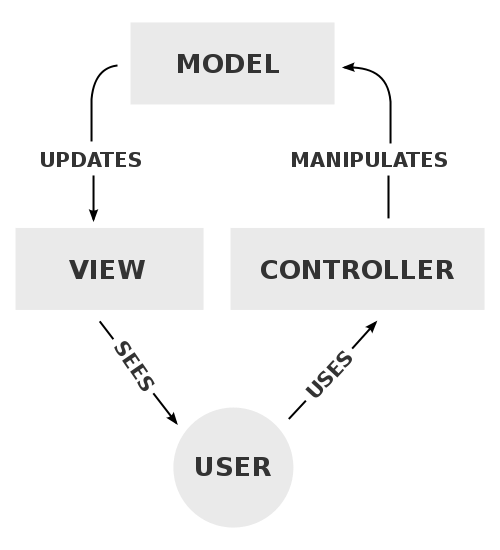
\includegraphics[scale=0.3]{./img/MVC.png}
\caption{\small{The Model, View and Controller, interconnected by directed edges}}
\label{mvc}
	
\end{figure}

As shown in fig \ref{mvc}, the MVC separates the application into a front end, the View, and a back end, the Model and Controller. The Controller provides the link between both the View and the Model, which makes it act as the brain of the application. The Controller decides what the user input was and how the Model needs to change as a result of this input\cite{codinghorror}. The Controller then responds back to the user by calling the resulting View.

\subsection{Choice of framework}
In order to be able to choose a suitable web application framework, we have defined some constraints for ourselves that we can use to benchmark various popular existing frameworks. Our first criteria was choosing a framework which would ideally be based on Java language that we learned during our education, especially noting the given time constraints. With this in mind, we narrowed our choices down to four popular frameworks such as \href{https://grails.org/}{Grails}, \href{https://vaadin.com/home}{Vaadin}, \href{https://www.playframework.com/}{Play!} and \href{http://projects.spring.io/spring-framework/}{Spring}. A second criteria was that it should be future proof, as the application would be extended as an open source project in the future. Comparing these frameworks in terms of popularity, supporting community and compatibility, we were able to boil down our choice to either the Spring framework or the Play! framework. A benchmarking between these two frameworks is shown in the table below.
\subsubsection{Benchmarking}
 The table below lists the comparison of these two frameworks within the constraints that we have defined:\\

\begin{figure}[h]
\centering
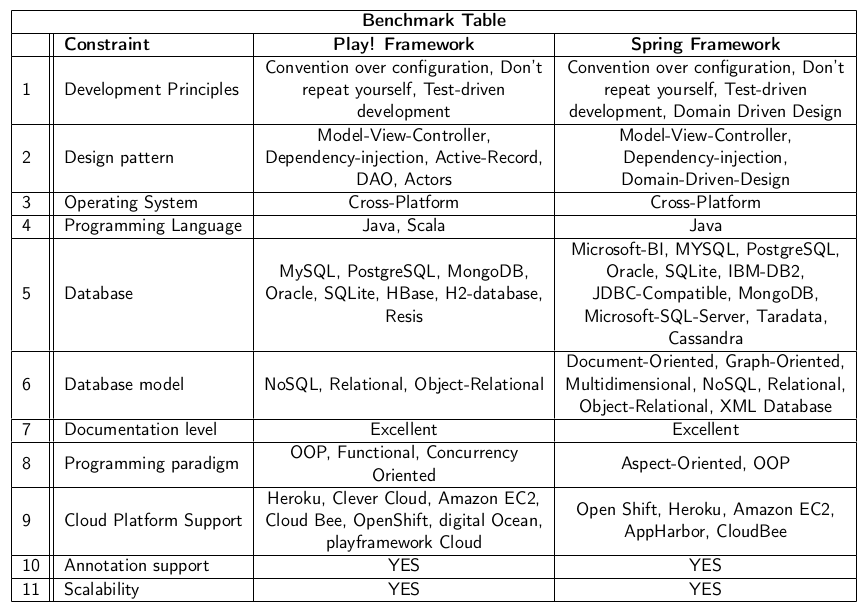
\includegraphics[scale=0.5]{./img/benchmark.png}	
\end{figure}


The result of this benchmark shows us that the differences between these two frameworks are fairly minimal. We decided to use the Play!Framework for this project because of the Scala support, the Programming paradigms and the Cloud Platform support.
\newpage

\subsection{Play! Framework}
  One of the main reasons we selected the Play! Framework is also because this framework has been proven in production. For example the LinkedIn web application has been developed using the Play! Framework. The following figure\ref{play} illustrates an overview of the Play! Framework.\\
\begin{figure}[h!]
\centering
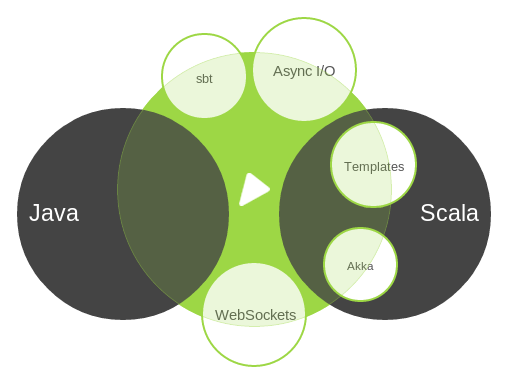
\includegraphics[scale=0.5]{./img/play.png}
\caption{\small{The main attributes and features of the Play! Framework}}
\label{play}
\end{figure}
 
 
The Play! Framework offers excellent documentation\cite{playDoc} that can help us get familiar with the Play! environment. First of all, it is an open source application that has an amazing error handling because of the fact that everything is compiled and built on the fly. This makes it easier for developers to detect bugs and can dramatically improve the developer's productivity to make changes. By reloading the browser, you can immediately see the changes you just made, which makes it perfect for fast prototyping within our project. Moreover, Play! supports both the Scala and Java languages, it comes with a Scala template that allows you to write dynamic code within an HTML body, and it also comes with pre-configured testing support. This last one is particularly important because that means we do not need to worry about adding JUnit dependencies to the build file. \\\\
Play! also offers the use of the EBean server interface which is very handy for fetching and saving beans to a particular DataSource. It can make reactive applications simpler because Play! is built on \href{http://netty.io/}{Netty}, which means it supports non-blocking I/O.\footnote{ non-blocking I/O is a form of input/output processing that permits other processing to continue before the transmission has finished.} This will enable our web application to make remote calls inexpensively which is crucial for high performance.

\section{Project Development Methodology} % (fold)

For our project development methodology we chose the agile Scrum methodology. This means that we will have weekly sprints (iterations within a fixed amount of time) in which a predefined set of items, taken from a product backlog\footnote{The agile product backlog in Scrum is a prioritized features list, containing short descriptions of all functionality desired in the product.\cite{backlog} }, are to be implemented. Each week we show our client what we achieved, and we discuss possible changes (within the requirements that have been agreed upon). The Scrum method gives developers an advantage over sequential methodologies such as the waterfall model or the V-model, because when changes have to be made to either pieces of code, features or even requirements, the sequential methodologies force the developers to revise (or even redo) everything that happened after the point where they were processed within the implementation. These sort of changes are more manageable within iterative methodologies such as Scrum. Scrum also allows developers to uncover designing constraints that may not have been obvious at the start of the implementation by giving them the opportunity to pivot after every sprint. \\\\
Given these advantages, the use of the Scrum method should be the most adequate for our project. When using Scrum, some roles and conventions have to be attributed, which are listed below:

\begin{enumerate}
	\item \textbf{Roles}
		\begin{itemize}
			\item Development lead: Arnaud Hambenne
			\item Scrum master/Dev Team: Soheil Jahanshahi
			\item Product owner: TU Delft Library R \& D group  (Babak Dehghenpour, Nicoleta Nastase)
			\item Coach: Alberto Bacchelli
		\end{itemize}
	\item \textbf{Conventions}	
\begin{itemize}
		\item Sprint duration: One week.
		\item Sprint Planning meeting: A weekly meeting that is used to prioritize the selected features for each sprint. 
		\item Sprint reflection report: A weekly evaluation where the estimated effort is compared to the actual effort that was needed to implement the chosen features, and where possible issues are documented. The evaluation takes place at the end of each Sprint.
		\item Daily Scrum meeting: A daily meeting between the developers which takes about 15 minutes.
		\item Sprint review meeting: A weekly meeting of about 15-20 minutes with the clients, in order to receive their feedback on the implemented features.
\end{itemize}
\end{enumerate}

\subsubsection{Definition of Done} 
In order to be sure that every component functions correctly, we narrow down the definition we use for the word `done'. When we say a function or the application is `done' we mean that it is: 

\begin{itemize}
	\item	Implemented (the code has been written)
	\item	Unit tested (JUnit test cases)
	\item 	Integrated
	\item 	Integration tested
	\item 	Documented (the change has been documented)
\end{itemize} 



